\section{Approach \& Uniqueness}

In order to enforce reservations while running BE jobs opportunistically, our
approach uses priority scheduling instead of weights.

Enforcing priorities requires fewer global runqueue searches than weights do,
because they only need to happen on \textit{class boundary crossings}: on
\exit{}, when a core switches to running lower class processes after having
previously been running high class, and on \entry{}, when a core enqueues a high
class process. These checks ensure that a core $c$ running a BE thread $t$ knows
that there are no queued LC threads anywhere: the \exit{} check ensures theres
none when starting to run $t$, and the \entry{} check ensures if one wake up
while running $t$ it will interrupt $t$.

\begin{figure}[t]
    \centering
    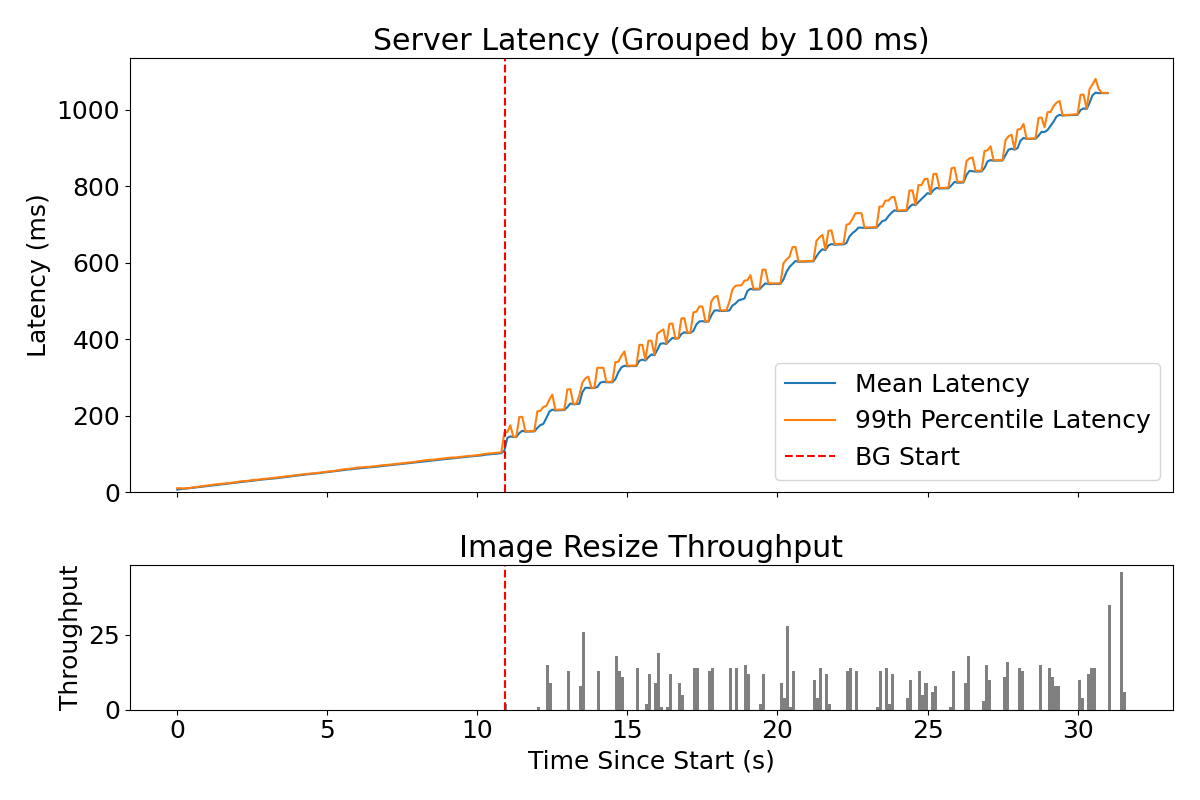
\includegraphics[width=\columnwidth]{graphs/overload-rt.png}
    \caption{when running the server in real time, throttling degrades
    its performance at high load}\label{fig:overload-rt}
\end{figure}


Linux enforces priority across scheduling classes, but higher class schedulers
are designed for real time applications. Additionally, if these experience high
load, Linux throttles them in order to not starve the default class. We see this
happening in \autoref{fig:overload-rt}, where throttling leads to spikes in the
BE task's throughput, and corresponding spikes in the server's latency.

We design a new scheduling class \beclass{} that sits at a lower priority than
the default, which enforces LC applications' uncontended access to CPUs they
reserved. To enforce reservations under high load, without throttling LCs or
killing BEs, \beclass{} is \textit{parked}, meaning the user-space code never
runs, only kernel-level services.